%!TEX root = THinstituteReport_1.tex

%\clearpage
%\newpage
%%%%%%%%%%%%%%%%%%%%%%%%%%%%%%%%%%%%%%%%%%
%\section{Robustness in heavy ion underlying event}
%\label{sec:robustness}
\subsection{Dissecting jet quenching observables using grooming}
\label{sec:dissecting}
%%%%%%%%%%%%%%%%%%%%%%%%%%%%%%%%%%%%%%%%%%

%\subsection{Subtraction algorithms}
%\label{sec:subtractionalgo}

%\subsection{Sensitivity to uncorrelated background}
%\label{sec:uncorrelatedbackground}
%
%The heavy ion background that is uncorrelated to the jet will populate the phase space in the form of soft splittings at large angle $\theta \approx R$, where the area is maximal. Depending on the considered jet $p_{T}$, these fake splittings can contribute significantly to the $z_{g}$ distribution by enhancing the number of asymmetric splittings and inducing a strong modification relative to vacuum jets. 
%Fig. \ref{fig:UncorrelatedBkg} shows the Lund diagram filled iteratively with PYTHIA jets embedded into a thermal background (left) and the difference plot to PYTHIA (right). The difference plot shows the enhancement of uncorrelated splittings at large angle. Superimposed to the plot, the black line with negative slope sets the limits for the subsample of splittings that would be selected by grooming with default parameters and highlights the fraction of fake splittings that would enter the $z_{g}$ calculation. The plot on the right is filled with jets at lower energies and shows that the impact of the uncorrelated background increases as expected.
%
%\begin{figure}[th]
%\centering
%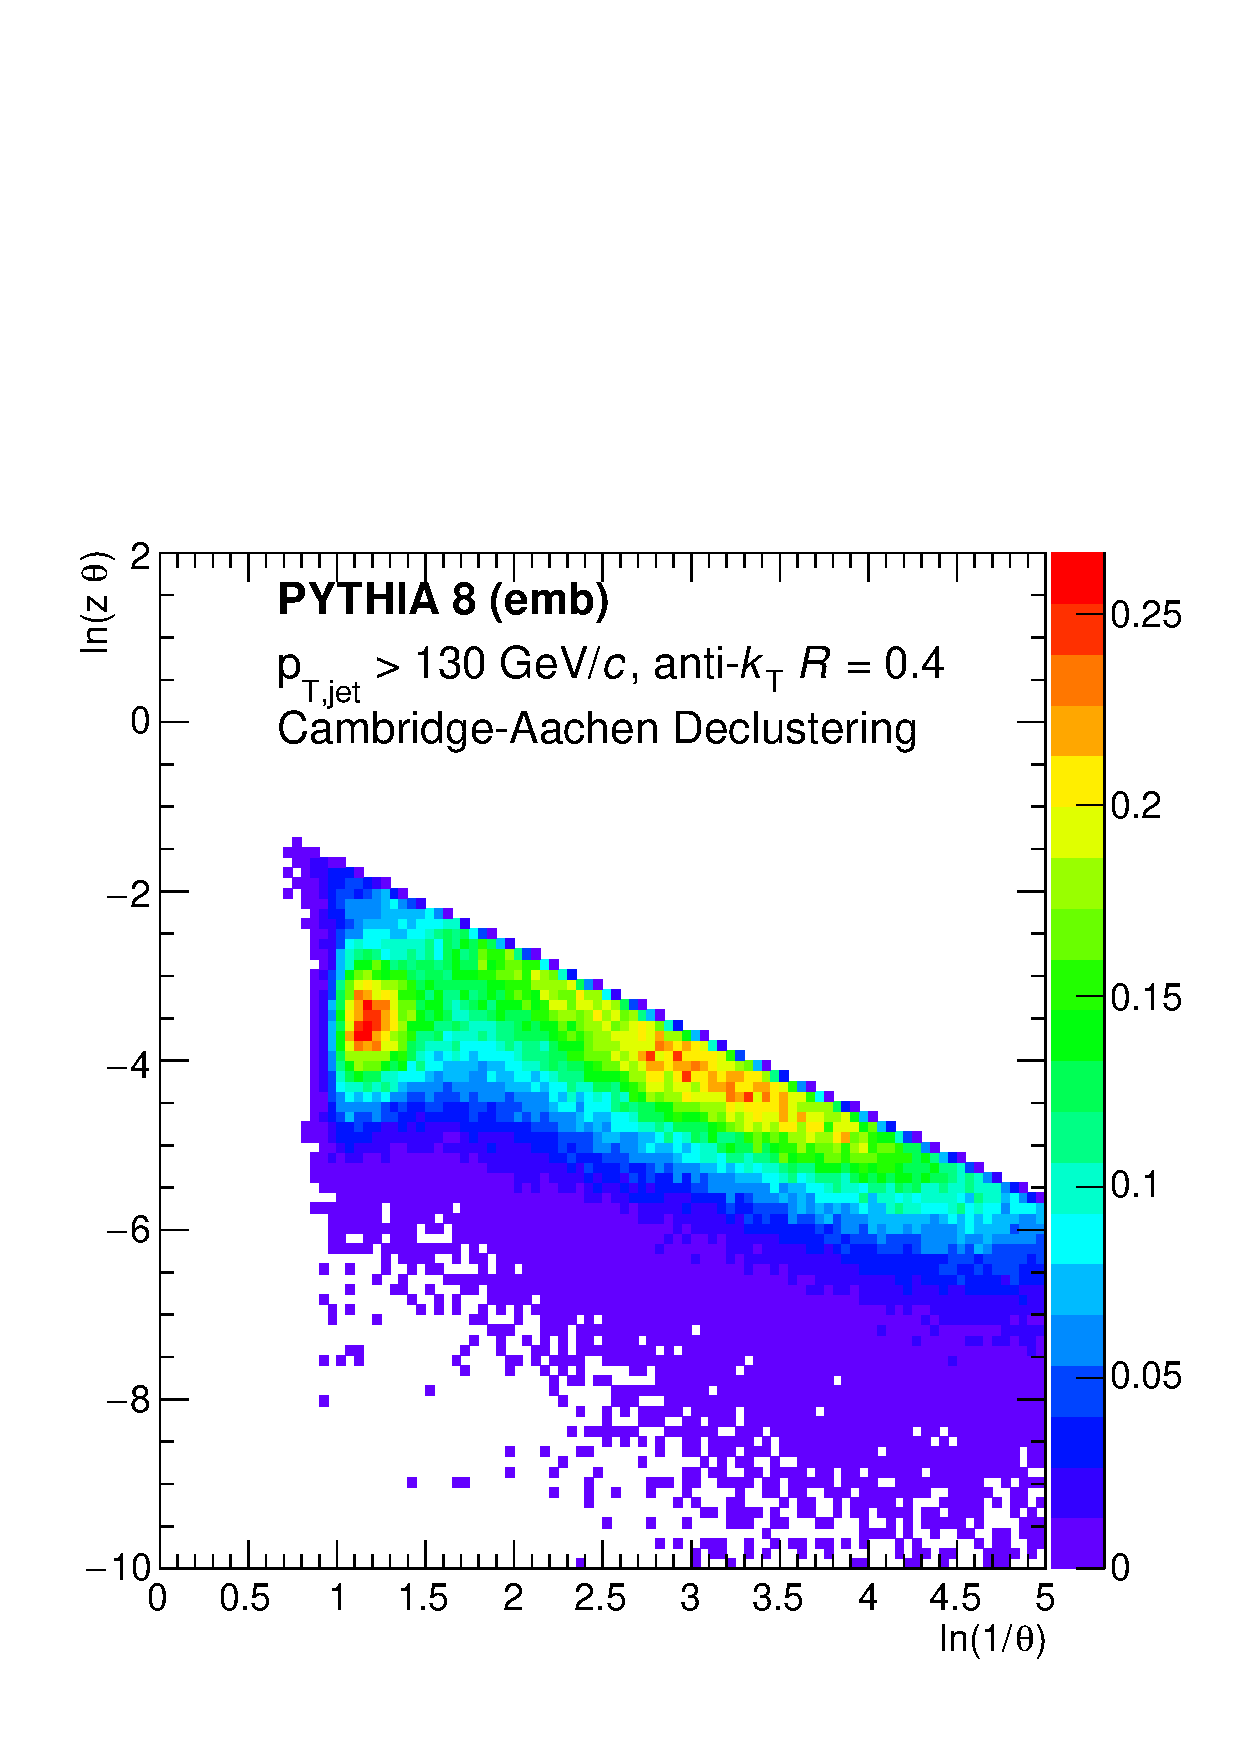
\includegraphics[width=0.4\textwidth]{figures/LundMC/Pyth_Emb.pdf}%
%%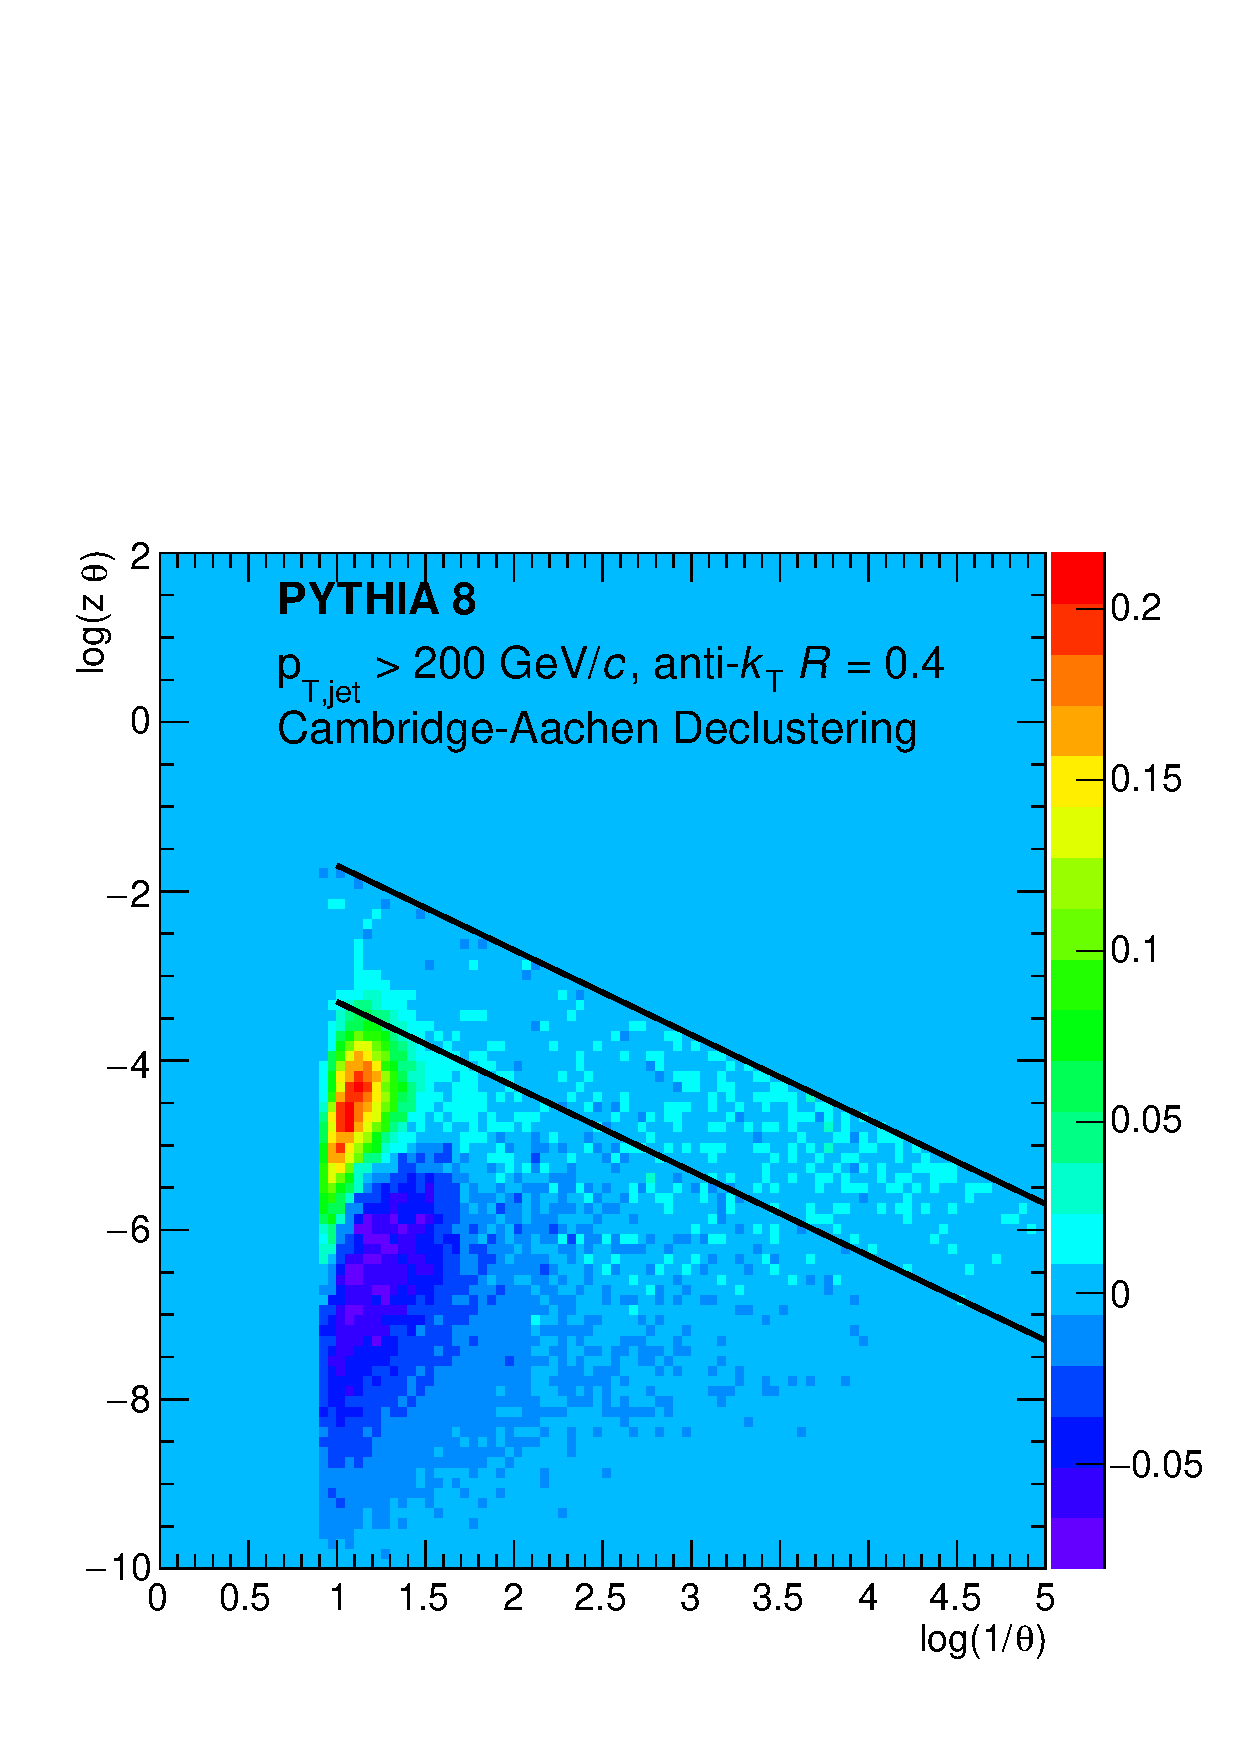
\includegraphics[width=0.33\textwidth]{figures/LundMC/PythiaDiffCA_wLines200.pdf}%
%%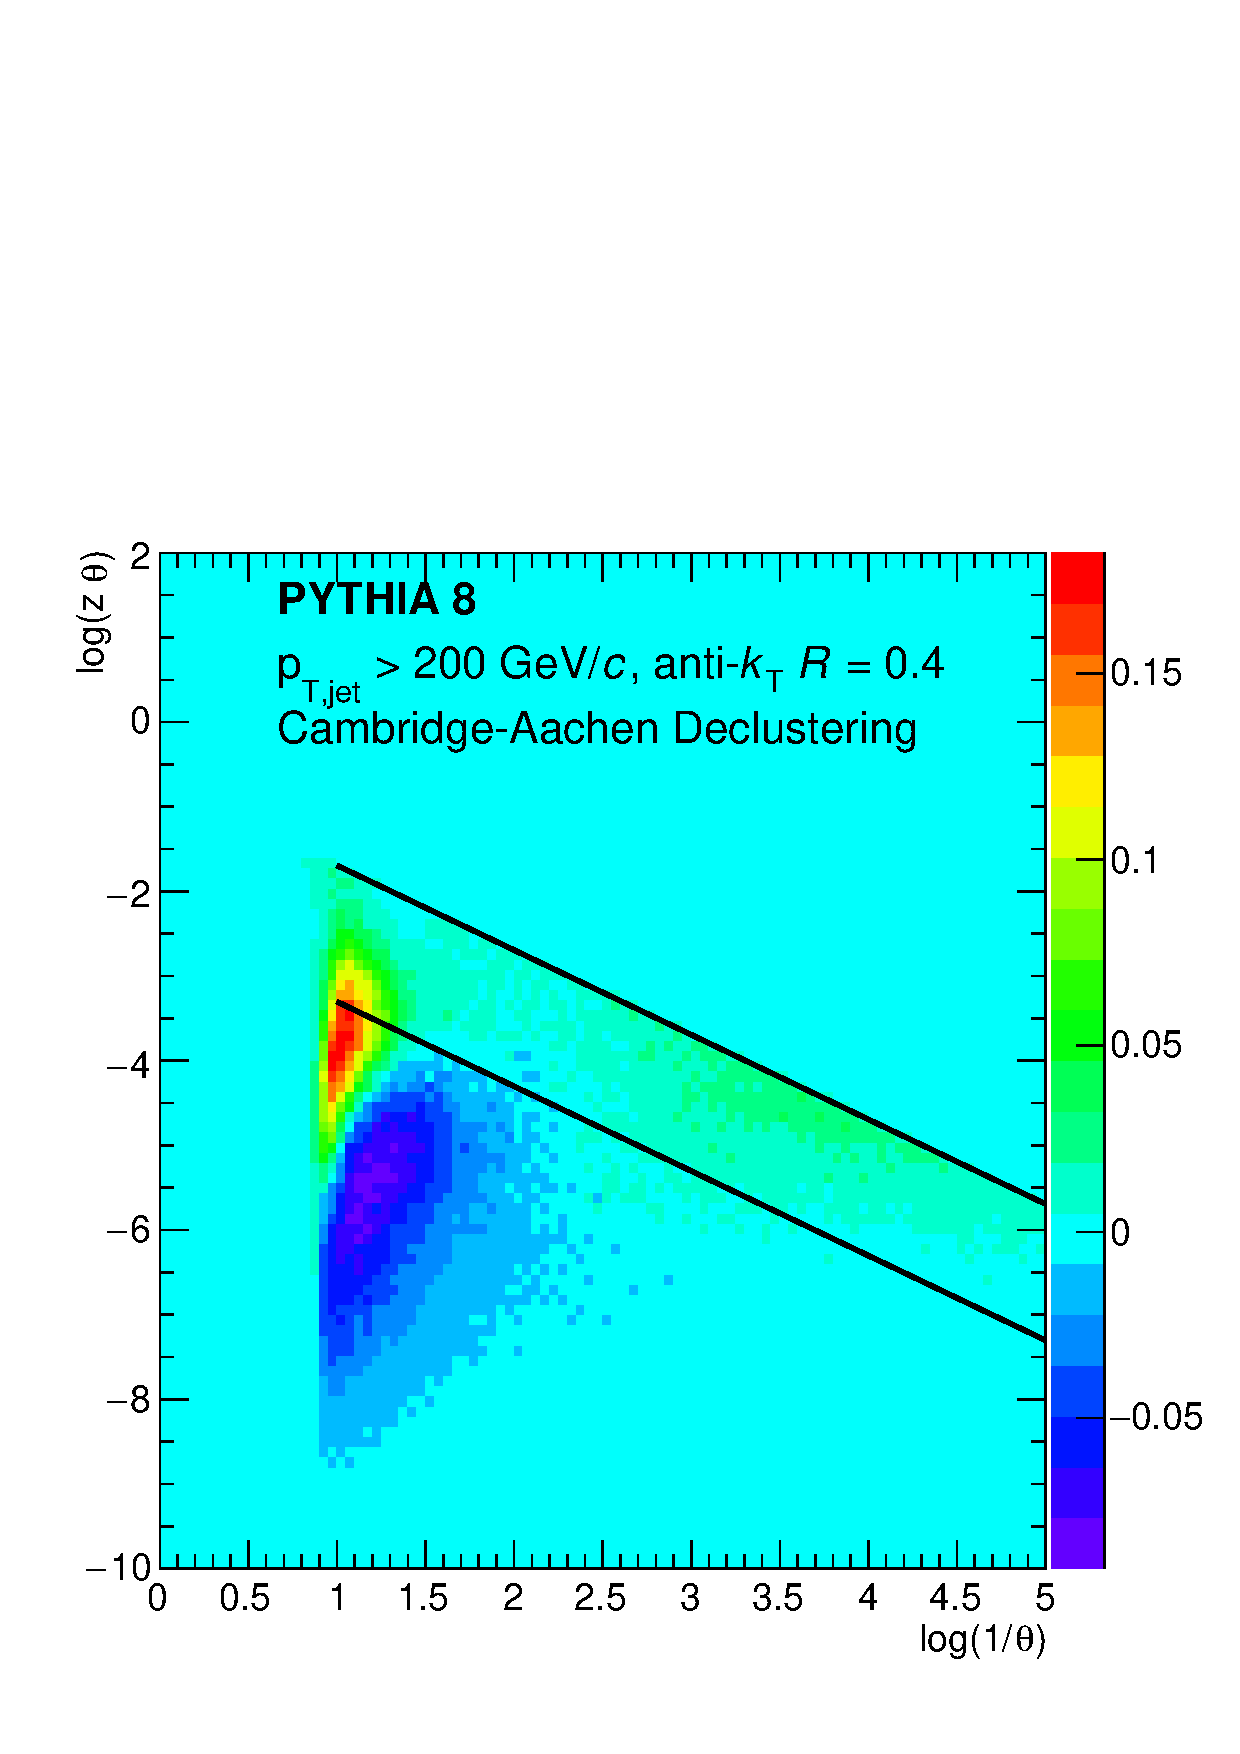
\includegraphics[width=0.33\textwidth]{figures/LundMC/PythiaDiffCA_wLines80120.pdf}%
%\caption{Impact of the uncorrelated background in the splitting map.}
%\label{fig:UncorrelatedBkg}
%\end{figure}
%Similar plots are shown for JEWEL and QPYTHIA in Fig.\ref{fig:UncorrelatedBkgSignal}. The plots correspond to JEWEL wo/recoils,JEWEL w/recoils and QPYTHIA, all embedded into a thermal background. We observe that after embedding, the difference to the vacuum reference(also embedded) is still significant, meaning that the differences in the fragmentation pattern from different generators survive to the presence of the Underlying Event. 
%
%\begin{figure}[th]
%\centering
%\includegraphics[width=0.33\textwidth]{figures/LundMC/JewelN1EmbeddedRecoilOff.pdf}%
%\includegraphics[width=0.33\textwidth]{figures/LundMC%/JewelN1EmbeddedDifference.pdf}%
%\caption{Impact of the uncorrelated background to the splitting map of JEWEL}
%\label{fig:UncorrelatedBkgJewel}
%\end{figure}

%\begin{figure}[th]
%\centering
%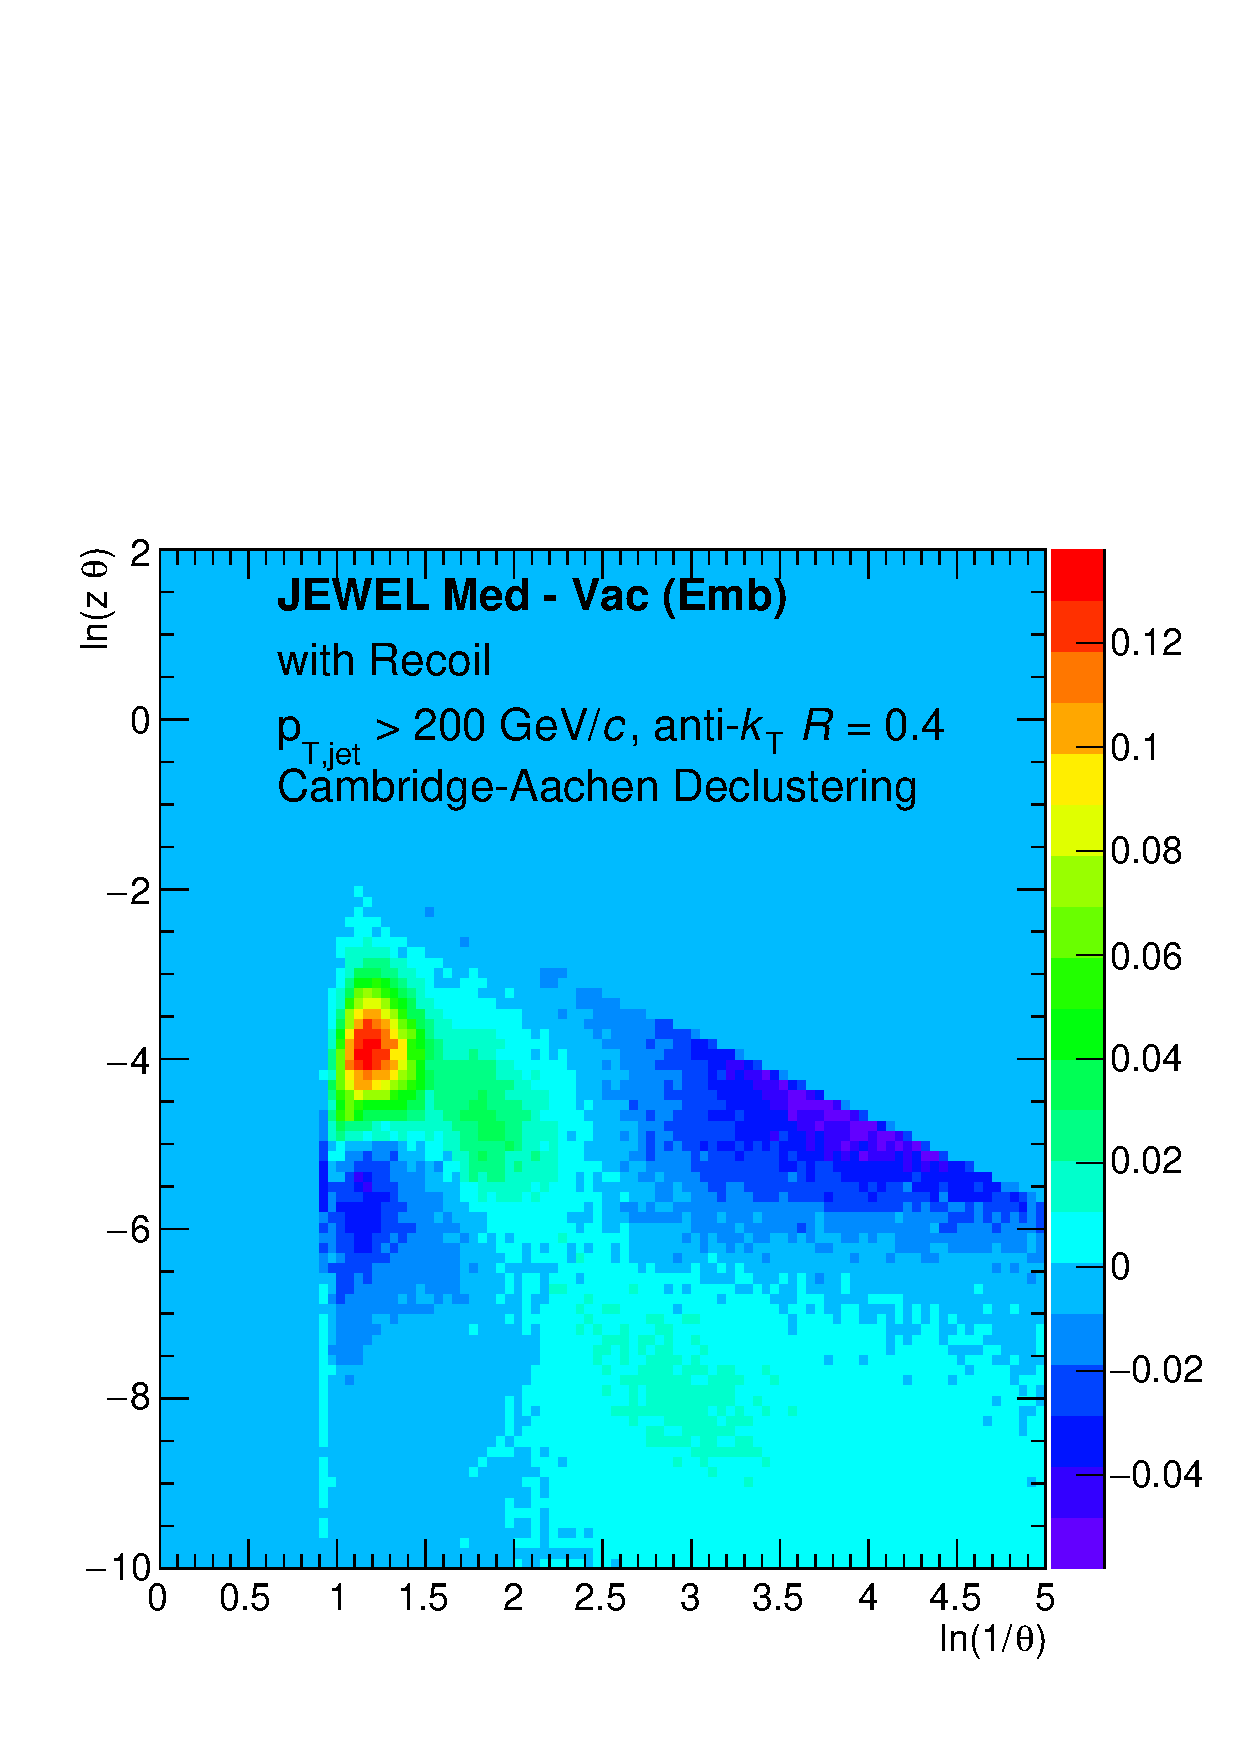
\includegraphics[width=0.33\textwidth]{figures/LundMC/JewelMedVacEmbeddedRecoilsOn.pdf}%
%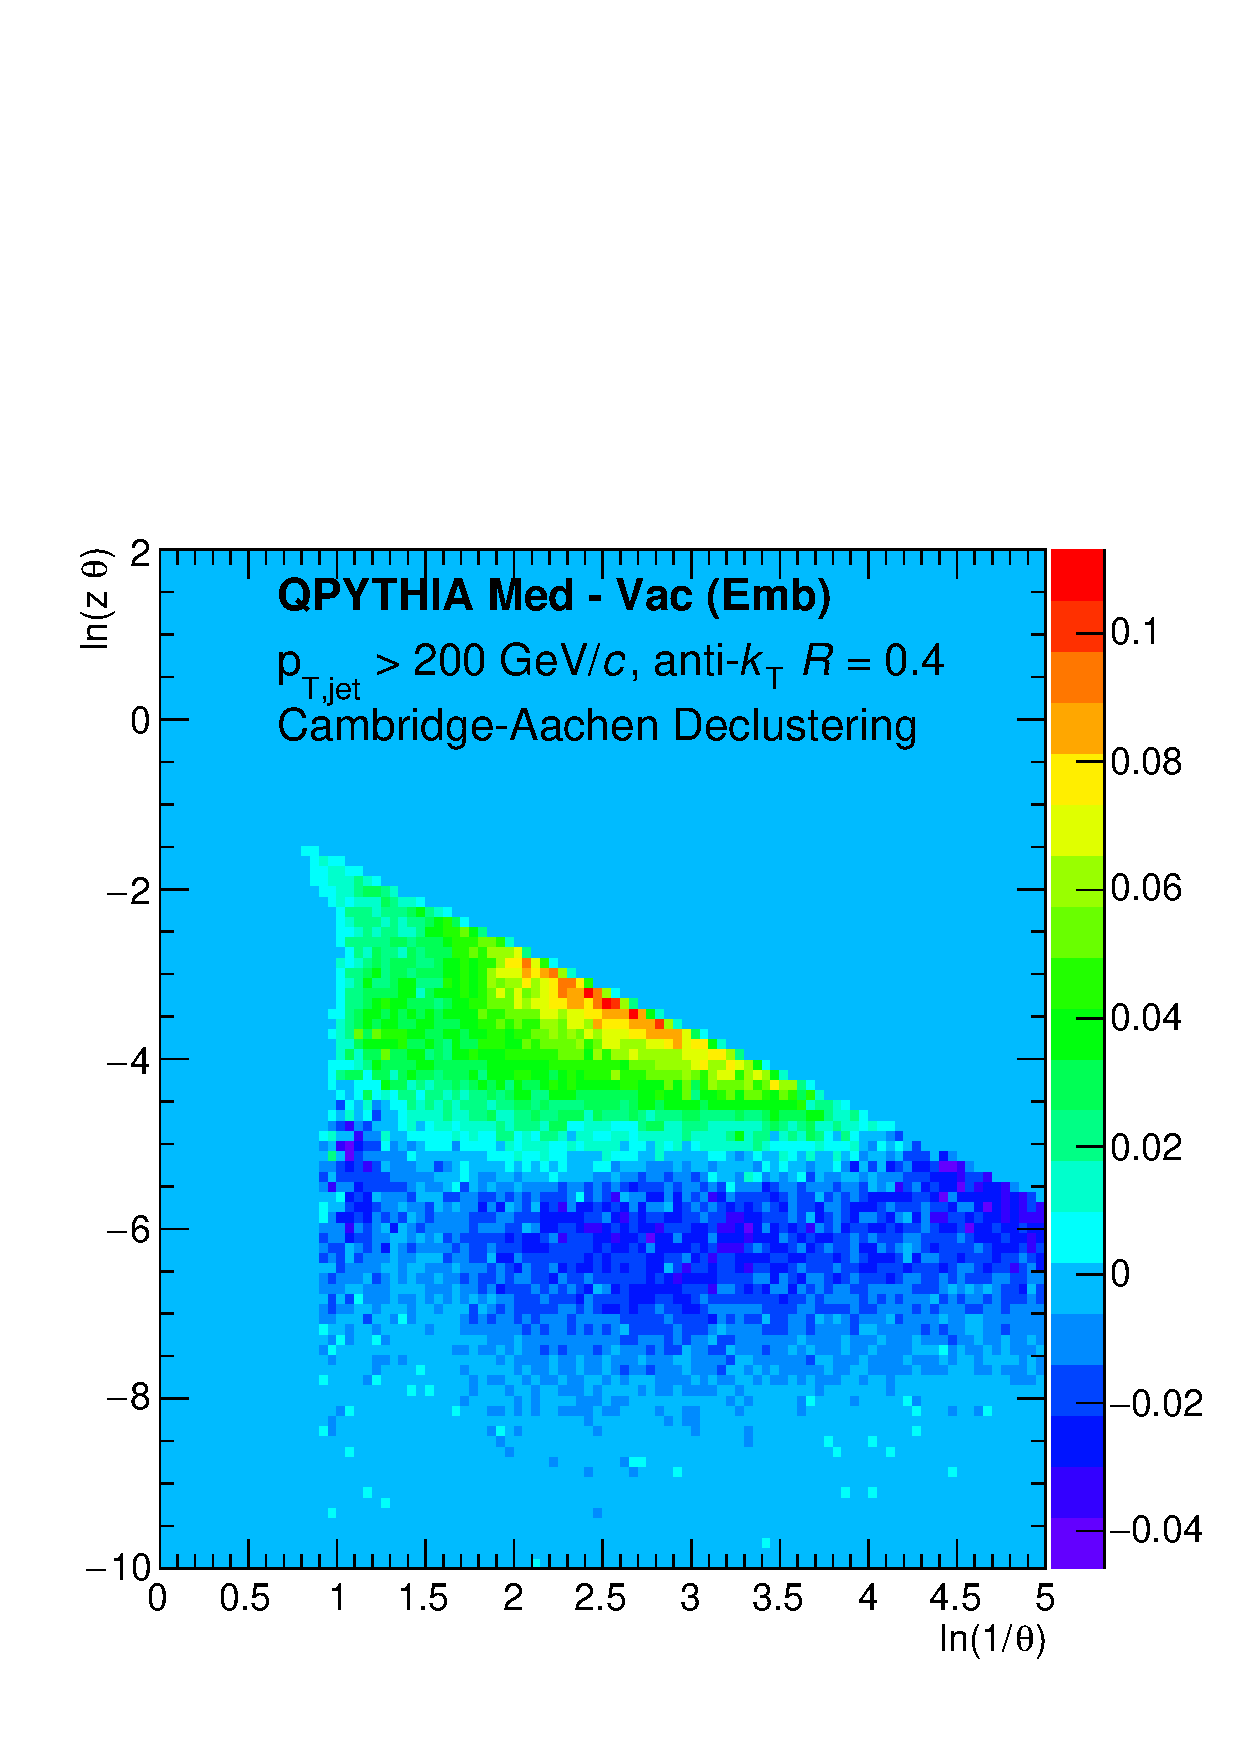
\includegraphics[width=0.33\textwidth]{figures/LundMC/QPythiaMedVacDiffEmbedded.pdf}
%\caption{Difference between the quenching MC embedded and the vacuum reference embedded. Left is JEWEL, right is QPYTHIA}
%\label{fig:UncorrelatedBkgSignal}
%\end{figure}

%\begin{figure}[th]
%\centering
%\includegraphics[width=0.33\textwidth]{figures/LundMC/RecursiveEmbeddedqpythia.pdf}%
%\includegraphics[width=0.33\textwidth]{figures/LundMC/RecursiveEmbeddedDifferenceqpythia.pdf}%
%\caption{Impact of the uncorrelated background to the splitting map of QPYTHIA}
%\label{fig:UncorrelatedBkgQPYTHIA}
%\end{figure}

%\subsection{Grooming-enhanced observables: examples}
In this section we present studies of conventional jet quenching observables that are enhanced by ``dissecting'' the jet samples using grooming techniques. As a first step, we have simply divided the fully inclusive sample according to the angle separating the two hardest prongs of a particular jet. These were, in turn, identified using SD grooming.
More importantly, all results in this section have been computed by embedding the MC jet samples into a realistic heavy-ion background that depends on centrality. Hence they represent more realistically the magnitude of effects that should be expected to arise in heavy-ion collisions at the LHC.

\begin{figure}[th]
\centering
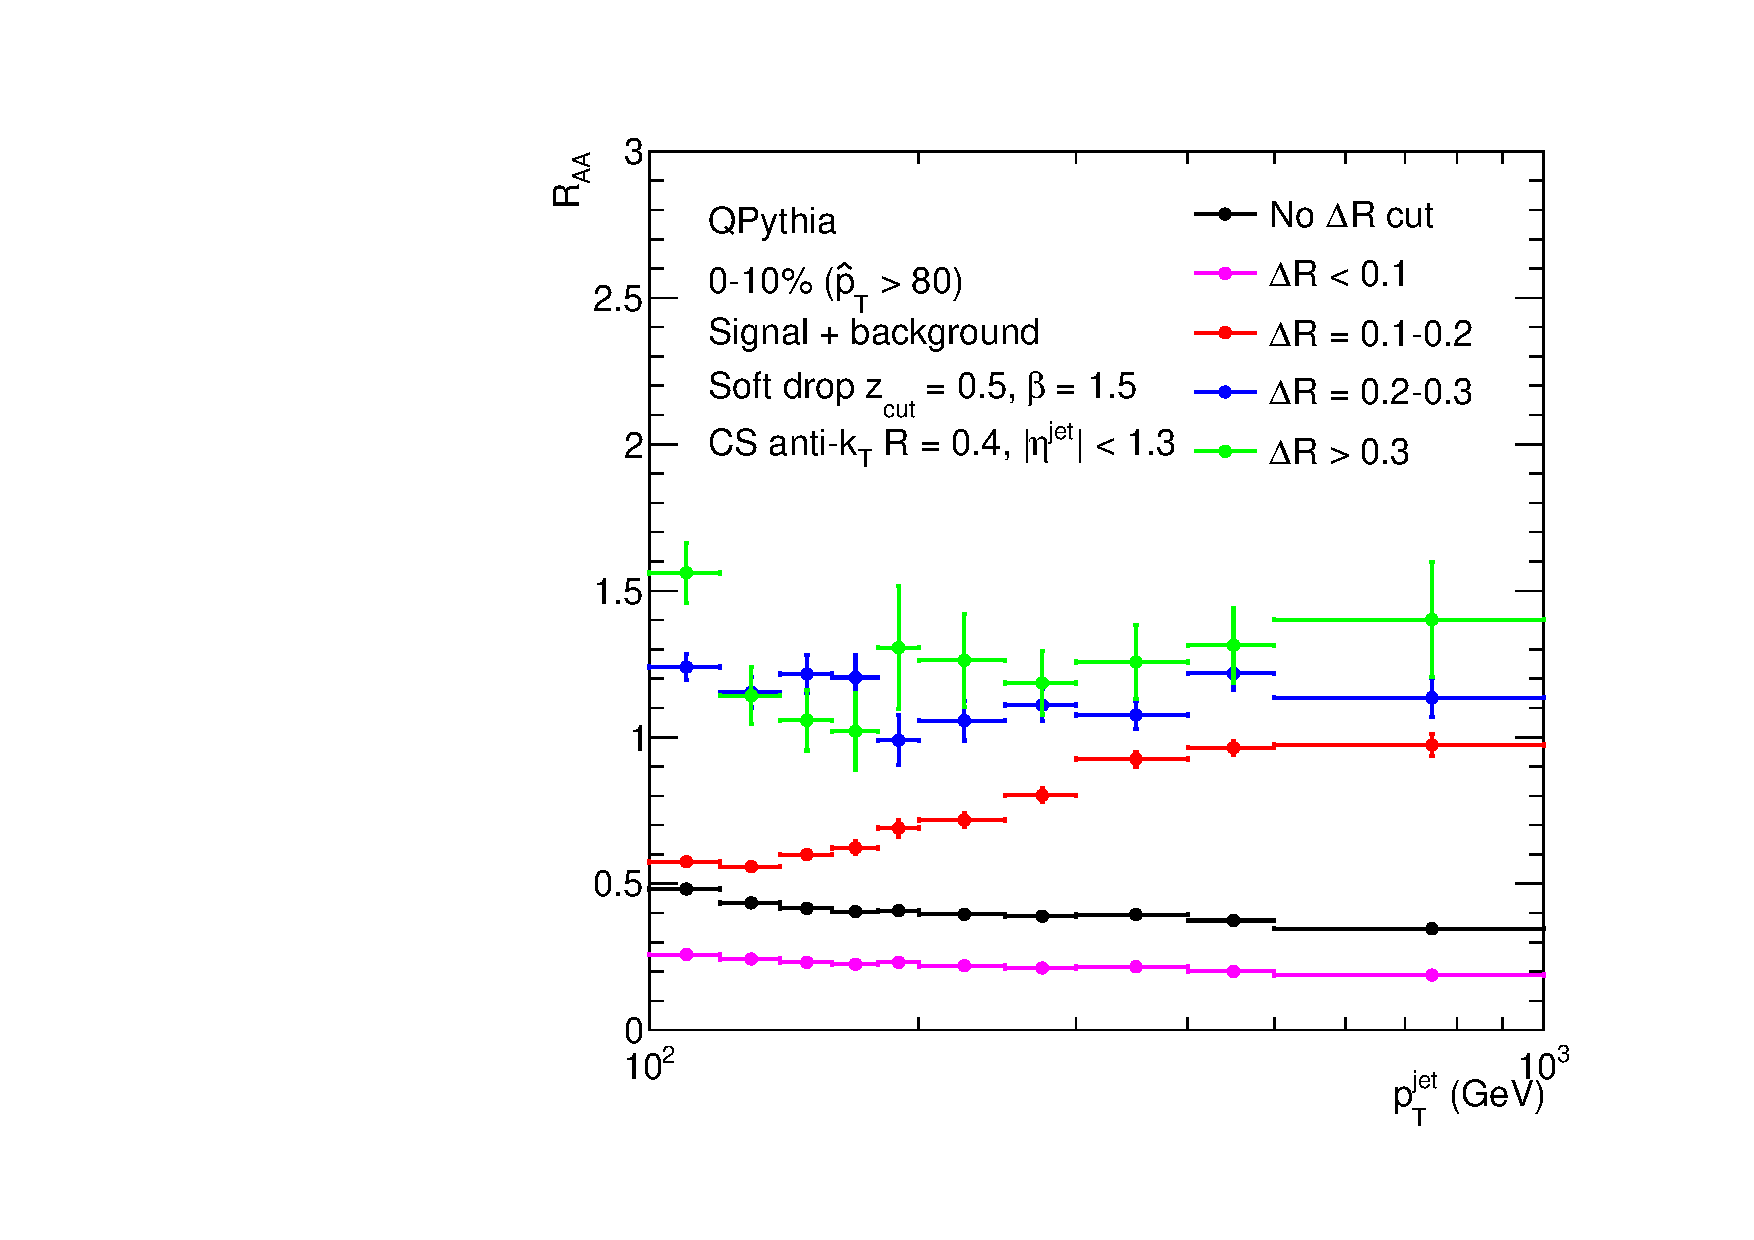
\includegraphics[width=0.45\textwidth]{figures/Observables_RAA/Plot9}%
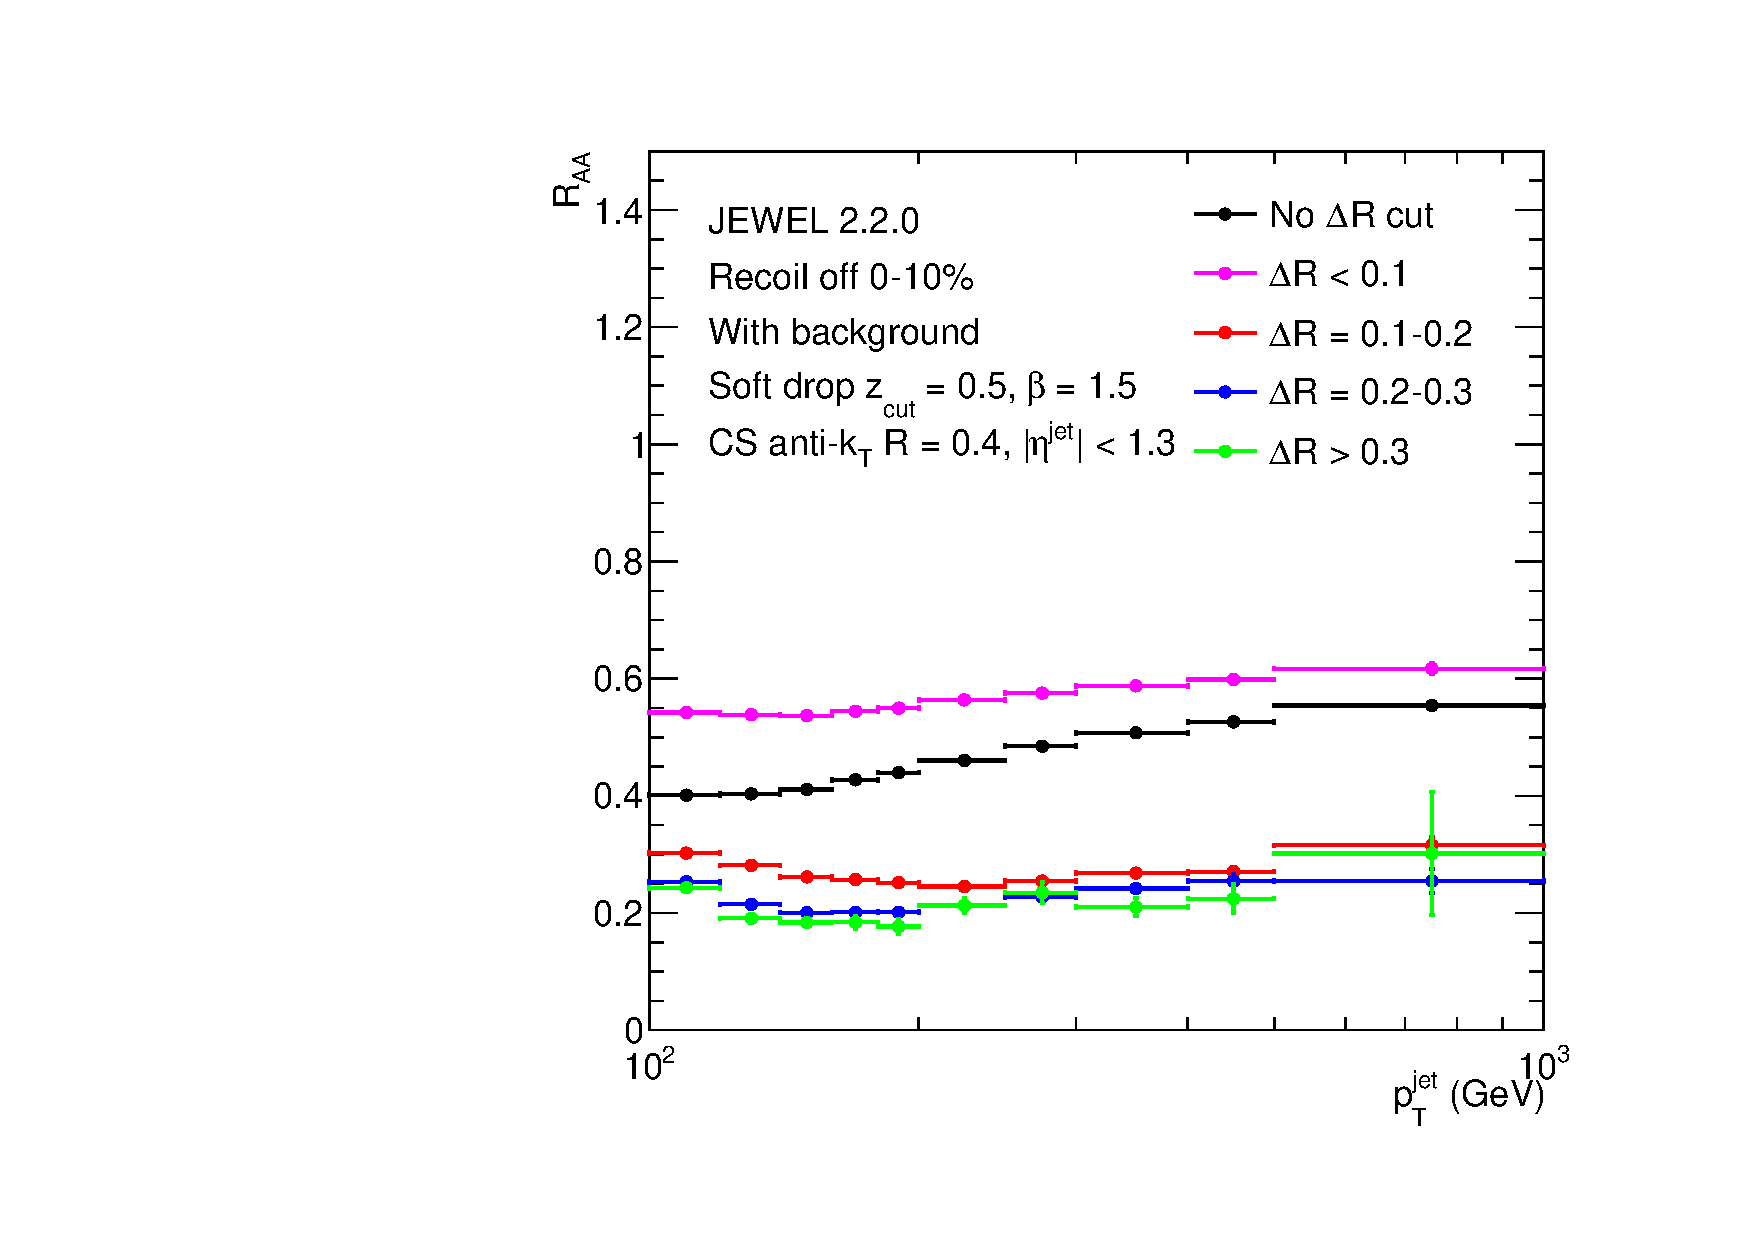
\includegraphics[width=0.45\textwidth]{figures/Observables_RAA/Plot3}\\
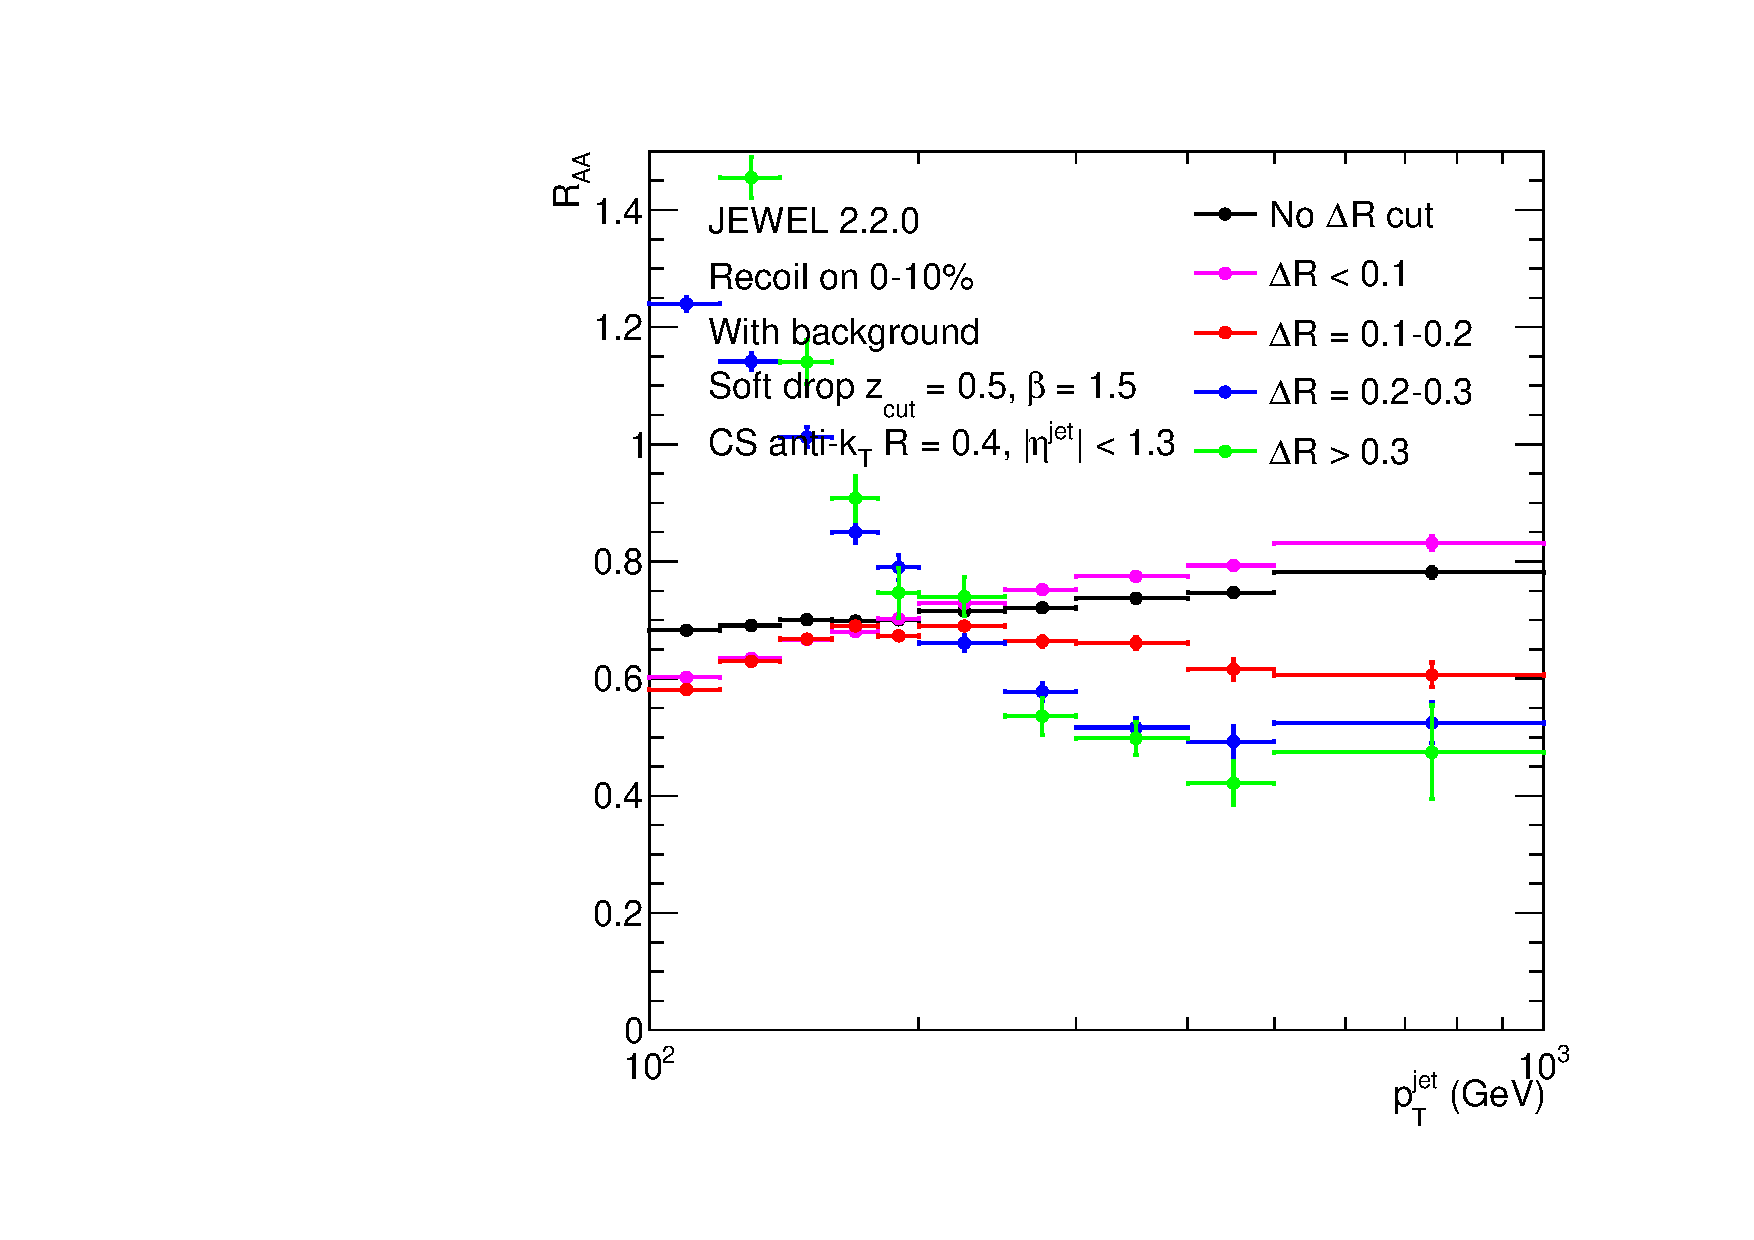
\includegraphics[width=0.45\textwidth]{figures/Observables_RAA/Plot4}
%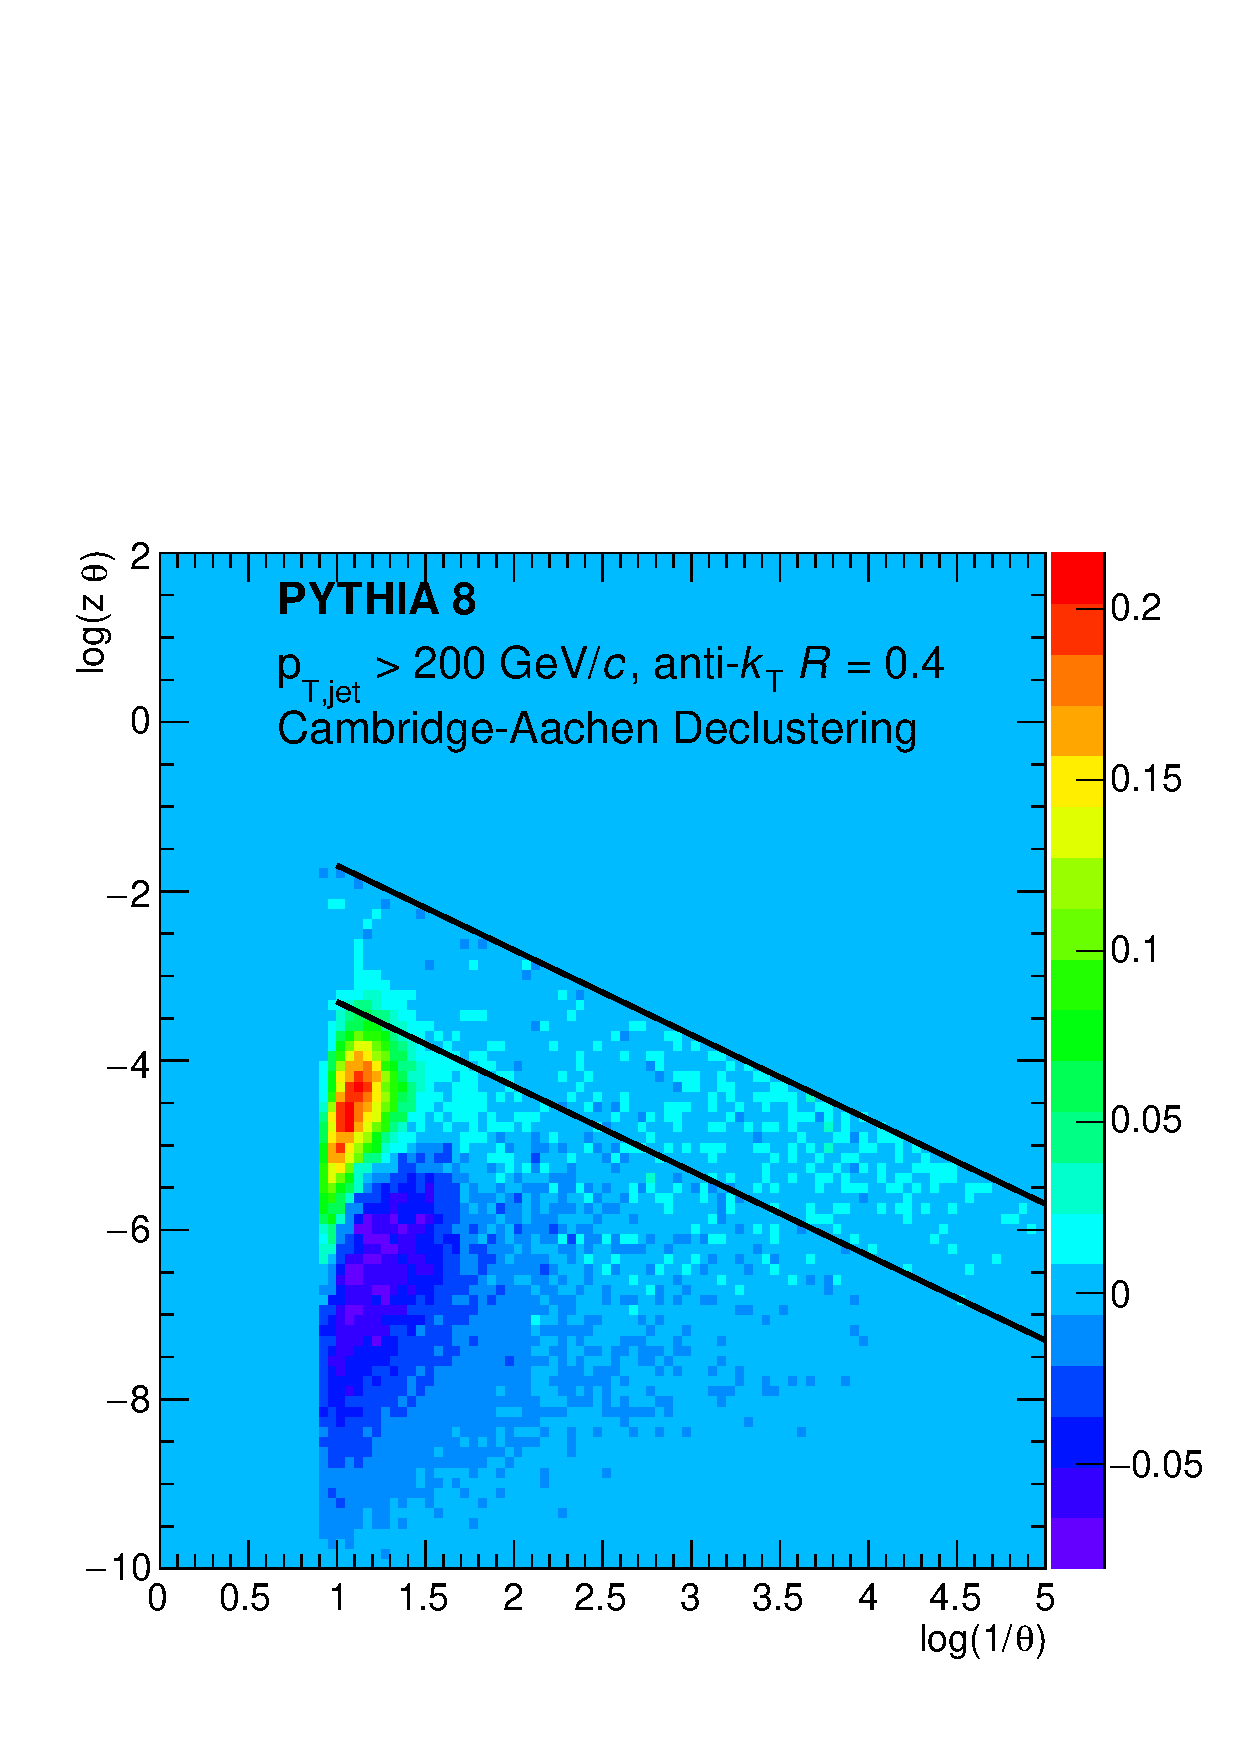
\includegraphics[width=0.33\textwidth]{figures/LundMC/PythiaDiffCA_wLines200.pdf}%
%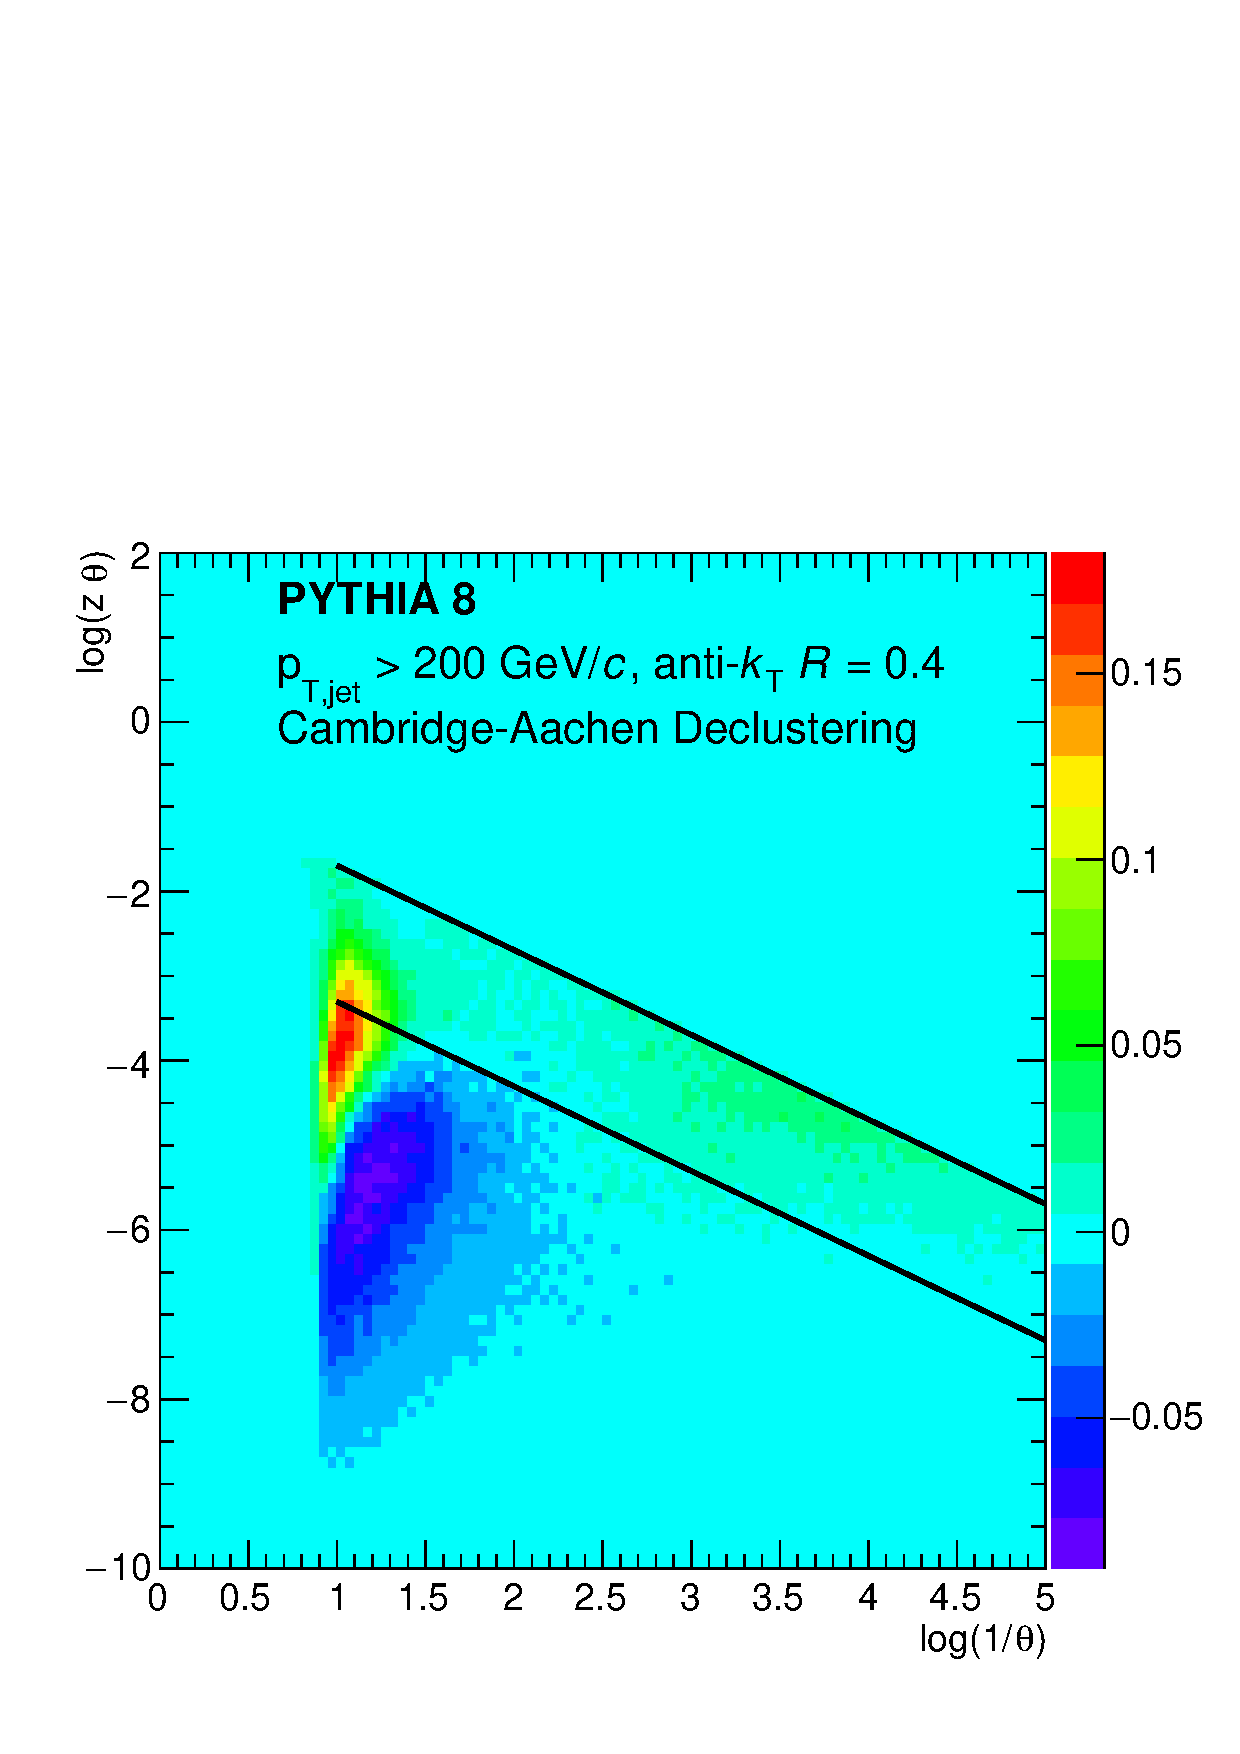
\includegraphics[width=0.33\textwidth]{figures/LundMC/PythiaDiffCA_wLines80120.pdf}%
\caption{The nuclear modification factor for subsamples of jets that have been unrolled as a function of the angle found between the leading sub-jets using SD. 
{\color{red} why aren't we sensitivity to the ``blob'' in recoil-off...?? which samples were used (new or old?)... old wasn't consistent with the publications..}
}
\label{fig:GroomedRAA}
\end{figure}
The famous nuclear modification factor, $R_{AA}$, is a standard benchmark for estimating/tuning medium parameters in jet quenching calculations. However, by dividing the sample of inclusive high-$\pT$ jets into small- and large-angle configurations using a particular grooming procedure (``dissecting'') we gain access to more information regarding the accompanying modifications of the intra-jet structure. Once again, this can be realized in many ways and below we will show results using SD.

The jet samples generated from QPYTHIA, JEWEL(recoil-off) and JEWEL that goes into calculating $R_{AA}$ in \autoref{fig:GroomedRAA}, has been divided using SD(0.5,1.5) grooming into samples related to the angular separation of the hardest branches. While all three models gives a similar $\pT$-trend of $R_{AA}$ for the fully inclusive sample (see black points in \autoref{fig:GroomedRAA}), large differences are seen for the ``dissected'' samples.\footnote{The overall magnitude of the inclusive $R_{AA}$ does not play a major role in this analysis.} In QPYTHIA, the core of the jet is quenched stronger than the periphery, as expected from previous studies above. For JEWEL(recoil-off), the effect is completely opposite: the jet core is quenched much less than large-angle splittings. This comes as no surprise in light  of other substructure observables that were analyzed above. Including recoil effects, the JEWEL sample implies an strong $\pT$-dependence of large-angle jets.

\begin{figure}[th]
\centering
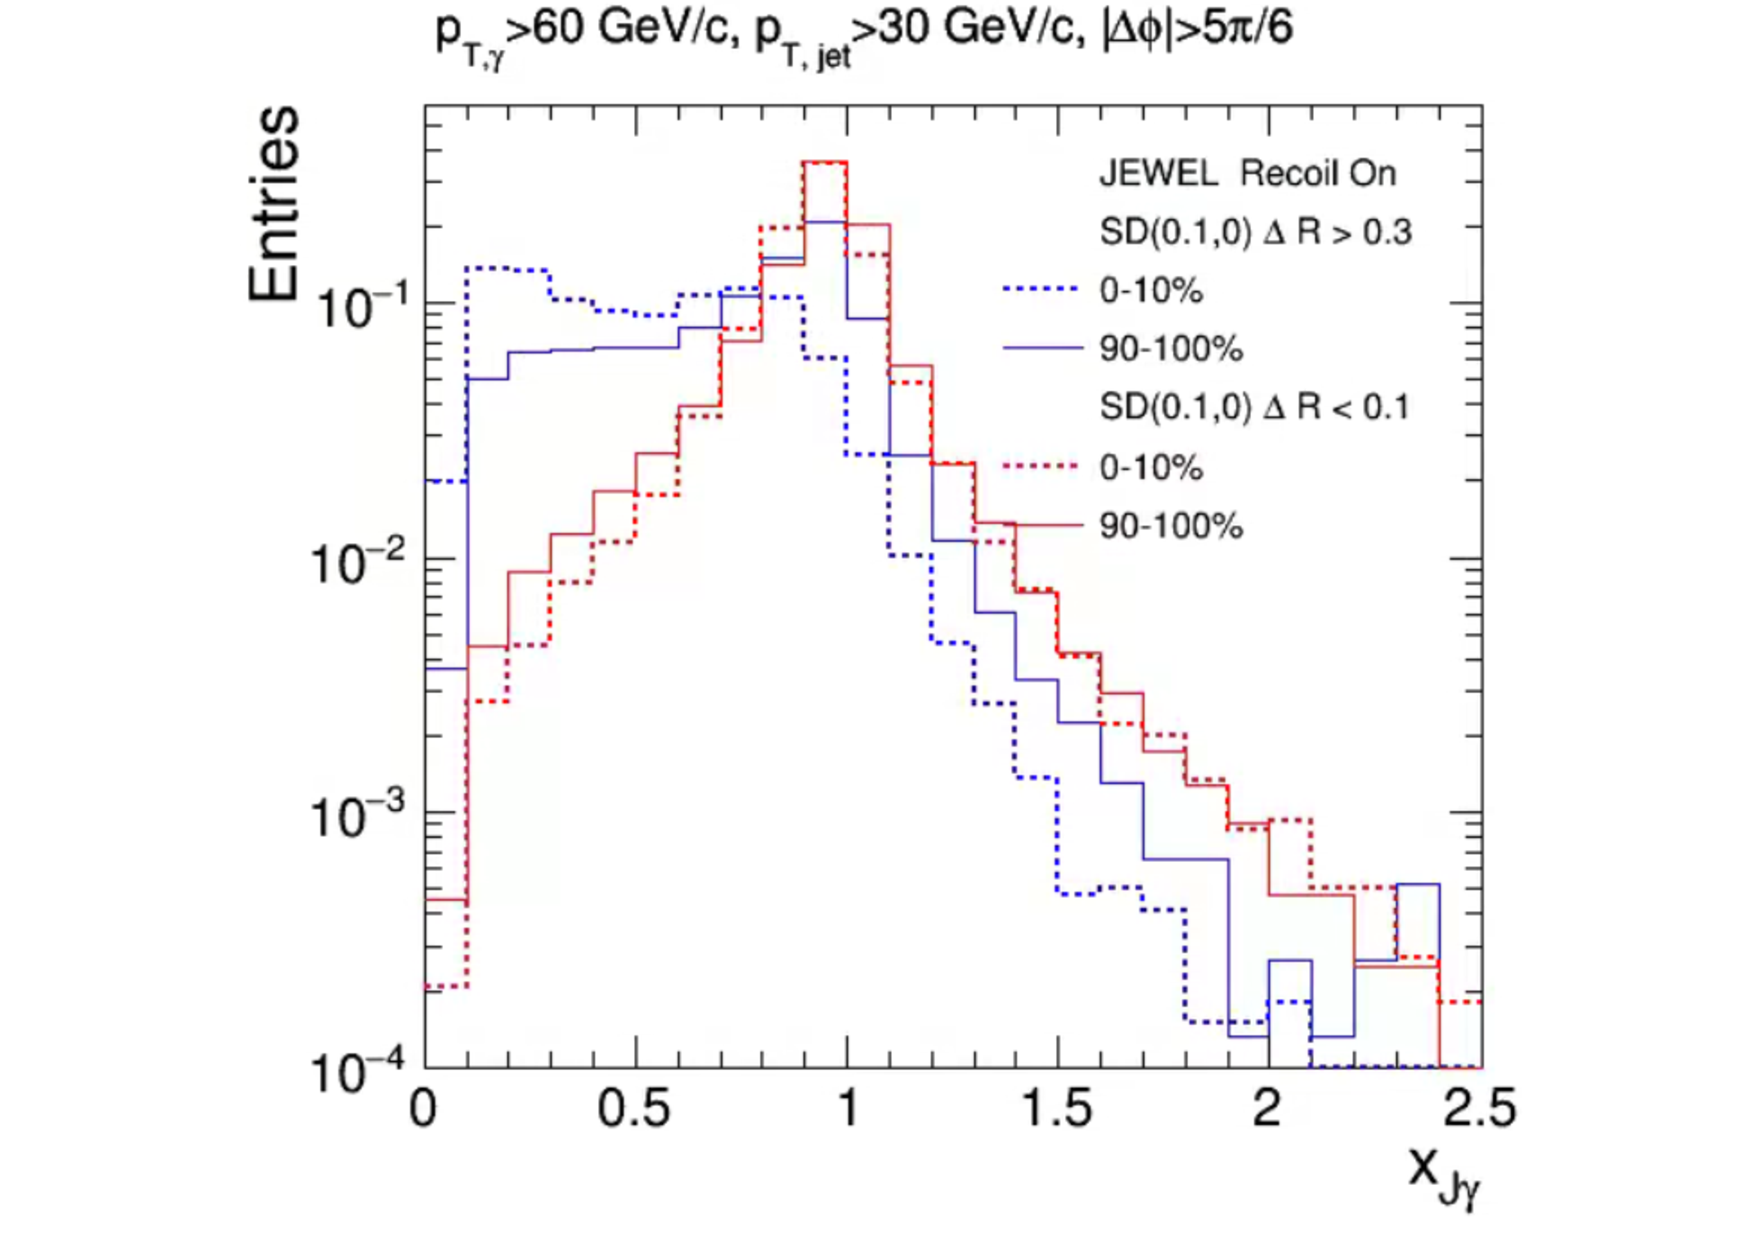
\includegraphics[width=0.5\textwidth]{figures/Observables_GammaJet/GammaJet_groomed}%
\caption{The $x_{J\gamma}$ distribution for subsamples of jets that have been unrolled as a function of the angle found between the leading sub-jets using SD. }
\label{fig:GroomedGammaJet}
\end{figure}
Another ``standard'' observables, is the gamma-jet asymmetry. 
In \autoref{fig:GroomedGammaJet} we have only included results for JEWEL, ``dissected'' as described above with SD(0.1,0) grooming. The same features that have been pointed out multiple times, also show up here as a function of collision centrality. While the small-angle sample shows little dependence of centrality, the large-angle sample evolves significantly from central to peripheral.

The results shown in this section are exploratory, and more systematic studies are left for future editions of the workshop.

\label{sec:observablesubtraction}